\documentclass[coursework]{SCWorks}
% Тип обучения (одно из значений):
%    bachelor   - бакалавриат (по умолчанию)
%    spec       - специальность
%    master     - магистратура
% Форма обучения (одно из значений):
%    och        - очное (по умолчанию)
%    zaoch      - заочное
% Тип работы (одно из значений):
%    coursework - курсовая работа (по умолчанию)
%    referat    - реферат
%  * otchet     - универсальный отчет
%  * nirjournal - журнал НИР
%  * digital    - итоговая работа для цифровой кафедры
%    diploma    - дипломная работа
%    pract      - отчет о научно-исследовательской работе
%    autoref    - автореферат выпускной работы
%    assignment - задание на выпускную квалификационную работу
%    review     - отзыв руководителя
%    critique   - рецензия на выпускную работу

% * Добавлены вручную. За вопросами к @mchernigin
\usepackage{preamble}

\begin{document}

% Кафедра (в родительном падеже)
\chair{математической кибернетики и компьютерных наук}

% Тема работы
\title{Разработка и программная реализация сбалансированных деревьев поиска для эффективного управления данными в среде Linux}

% Курс
\course{1}

% Группа
\group{111}

% Факультет (в родительном падеже) (по умолчанию "факультета КНиИТ")
% \department{факультета КНиИТ}

% Специальность/направление код - наименование
\napravlenie{02.03.02 "--- Фундаментальная информатика и информационные технологии}
% \napravlenie{02.03.01 "--- Математическое обеспечение и администрирование информационных систем}
% \napravlenie{09.03.01 "--- Информатика и вычислительная техника}
% \napravlenie{09.03.04 "--- Программная инженерия}
% \napravlenie{10.05.01 "--- Компьютерная безопасность}

% Для студентки. Для работы студента следующая команда не нужна.
% \studenttitle{студентки}

% Фамилия, имя, отчество в родительном падеже
\author{Яшина Егора Алексеевича}

% Заведующий кафедрой
\chtitle{доцент, к.\,ф.-м.\,н.}
\chname{С.\,В.\,Миронов}

% Руководитель ДПП ПП для цифровой кафедры (перекрывает заведующего кафедры)
% \chpretitle{
%     заведующий кафедрой математических основ информатики и олимпиадного\\
%     программирования на базе МАОУ <<Ф"=Т лицей №1>>
% }
% \chtitle{г. Саратов, к.\,ф.-м.\,н., доцент}
% \chname{Кондратова\, Ю.\,Н.}

% Научный руководитель (для реферата преподаватель проверяющий работу)
\satitle{доцент, к.\,ф.-м.\,н.} %должность, степень, звание
\saname{Г.\,Г.\,Наркайтис}

% Руководитель практики от организации (руководитель для цифровой кафедры)
\patitle{доцент, к.\,ф.-м.\,н.}
\paname{С.\,В.\,Миронов}

% Руководитель НИР
\nirtitle{доцент, к.\,п.\,н.} % степень, звание
\nirname{В.\,А.\,Векслер}

% Семестр (только для практики, для остальных типов работ не используется)
\term{2}

% Наименование практики (только для практики, для остальных типов работ не
% используется)
\practtype{учебная}

% Продолжительность практики (количество недель) (только для практики, для
% остальных типов работ не используется)
\duration{2}

% Даты начала и окончания практики (только для практики, для остальных типов
% работ не используется)
\practStart{01.07.2024}
\practFinish{13.01.2024}

% Год выполнения отчета
\date{2024}

\maketitle

% Включение нумерации рисунков, формул и таблиц по разделам (по умолчанию -
% нумерация сквозная) (допускается оба вида нумерации)
\secNumbering

\tableofcontents

% Раздел "Обозначения и сокращения". Может отсутствовать в работе
% \abbreviations
% \begin{description}
%     \item ... "--- ...
%     \item ... "--- ...
% \end{description}

% Раздел "Определения". Может отсутствовать в работе
% \definitions

% Раздел "Определения, обозначения и сокращения". Может отсутствовать в работе.
% Если присутствует, то заменяет собой разделы "Обозначения и сокращения" и
% "Определения"
% \defabbr

\intro

В современных операционных системах на базе Linux эффективное управление динамическими структурами данных является критически важным для обеспечения высокой производительности системного программного обеспечения. При работе с большими объемами информации стандартные линейные структуры, такие как массивы или связанные списки, демонстрируют неудовлетворительное время выполнения базовых операций поиска, вставки и удаления. Для оптимизации этих процессов применяются самобалансирующиеся бинарные деревья поиска. В данной работе рассматривается практическая реализация Красно"=черного дерева на языке C++ с интеграцией автоматизированных скриптов тестирования производительности на языке Python.
% После введения — серии \section, \subsection и т.д.

\section{Теоретические основы и математические модели}

Красно"=черное дерево "--- это один из видов самобалансирующихся бинарных деревьев поиска, гарантирующий, что время выполнения основных операций не превышает логарифмического предела от количества элементов~\cite{cormen2013}.

Каждый узел дерева содержит дополнительное поле цвета (красный или черный) и удовлетворяет следующим свойствам~\cite{knuth2007}:

\begin{itemize}
    \item
        каждый узел является либо красным, либо черным;
    \item
        корень дерева всегда остается черным;
    \item
        все листья, не содержащие данных (олицетворяющие пустые указатели), являются черными;
    \item
        если узел красный, то оба его дочерних узла должны быть черными;
    \item
        любой простой путь от узла"=предка до заменяющего его листа"=потомка содержит одинаковое количество черных узлов.
\end{itemize}

Для оценки эффективности сбалансированного дерева введем математическую модель зависимости высоты дерева от общего числа узлов.

\begin{equation}
\label{eq:height_bound}
    h \le 2 \log_2(n+1)
\end{equation}

% \label{eq:height_bound}

Из данной модели следует, что временная сложность операции поиска в худшем случае составит $O(\log n)$.\

В процессе балансировки при вставке нового элемента ключевой операцией является локальный поворот поддерева. Важно отметить, что любые модификации и вращения структуры должны строго выполняться относительно родительского узла во избежание нарушения целостности указателей.\

Для сравнения эффективности также рассмотрим среднее количество поворотов при операции вставки, которое выражается через суммарный статистический предел.

\begin{equation}
\label{eq:average_rotations}
    E(R) = \sum_{i=1}^{k} p_i \cdot r_i = \frac{1}{N} \sum_{j=1}^{N} \Delta R_j
\end{equation}


\section{Архитектура и программная реализация}

Программный комплекс разделен на два основных модуля. Первый модуль написан на языке высокого уровня C++ и представляет собой системную библиотеку для работы со структурами данных в среде операционных систем на базе ядра Linux~\cite{tanenbaum2015}. Второй модуль реализован на языке Python и выполняет функции генерации тестовых наборов данных и визуализации метрик.

При проектировании класса дерева были определены основные переменные для управления указателями узлов: \texttt{root}, \texttt{parent} и \texttt{left}.\

Основной алгоритмический упор сделан на функцию вращения поддерева. Ниже представлена реализация метода левого поворота.

\begin{figure}[h!]
\caption{Реализация операции левого поворота поддерева на языке C++}
\label{code:left_rotate}
\begin{minted}[fontsize=\small, linenos=true, frame=single, breaklines=true]{cpp}
void LeftRotate(Node*& root, Node* x) {
    Node* y = x->right;
    x->right = y->left;
    if (y->left != nullptr) {
        y->left->parent = x;
    }
    y->parent = x->parent;
    if (x->parent == nullptr) {
        root = y;
    } else if (x == x->parent->left) {
        x->parent->left = y;
    } else {
        x->parent->right = y;
    }
    y->left = x;
    x->parent = y;
}
\end{minted}
\end{figure}

Как можно увидеть из исходного кода~\ref{code:left_rotate}, операция переприсваивания указателей требует атомарности логики во избежание утечек памяти в среде Linux.\

\begin{figure}[h!]
\caption{Скрипт автоматизации сборки и запуска тестовых сценариев на языке Bash}
\label{code:build_script}
\begin{minted}[fontsize=\small, linenos=true, frame=single, breaklines=true]{bash}
#!/bin/bash

# Скрипт автоматизации тестирования Красно-черного дерева
echo "=== Запуск сборки проекта ==="

# Компиляция исходного кода C++ с оптимизацией O3
g++ -O3 main.cpp -o rbtree_test

if [ $? -eq 0 ]; then
    echo "Компиляция успешно завершена."
    echo "Запуск анализа времени выполнения..."
    ./rbtree_test > test_results.log
    echo "Тестирование окончено. Результаты сохранены в test_results.log"
else
    echo "Ошибка компиляции!" >&2
    exit 1
fi
\end{minted}
\end{figure}

\section{Результаты экспериментов и сравнительный анализ}

Для подтверждения теоретических оценок сложности было проведено практическое тестирование разработанной реализации. Сравнение производилось со стандартным несбалансированным бинарным деревом поиска при последовательной вставке упорядоченного массива данных.\

Результаты замеров времени выполнения в микросекундах сведены в общую таблицу.\

\begin{table}[H]
\centering
\caption{Сравнительный анализ времени выполнения операций поиска в БДП и КЧД}
\label{tab:performance_results}
\begin{tabular}{|p{4cm}|>{\centering\arraybackslash}p{4.5cm}|>{\centering\arraybackslash}p{4.5cm}|}
\hline
\textbf{Количество узлов} & \textbf{Время БДП (мкс)} & \textbf{Время КЧД (мкс)} \\ \hline
100                       & 12                       & 5                        \\ \hline
500                       & 85                       & 9                        \\ \hline
1000                      & 194                      & 11                       \\ \hline
5000                      & 1120                     & 14                       \\ \hline
10000                     & 4380                     & 16                       \\ \hline
\end{tabular}
\end{table}

На основании данных, представленных в таблице~\ref{tab:performance_results}, можно сделать вывод о явной деградации производительности обычного бинарного дерева до линейной сложности при сохранении логарифмического времени у Красно"=черного дерева. Это наглядно иллюстрирует график распределения нагрузки, приведенный на рисунке~\ref{fig:chart_performance}.

\begin{figure}[h!]
\caption{Сравнительный анализ времени поиска (мкс) в зависимости от количества узлов}
\label{fig:chart_performance}
\begin{center}
    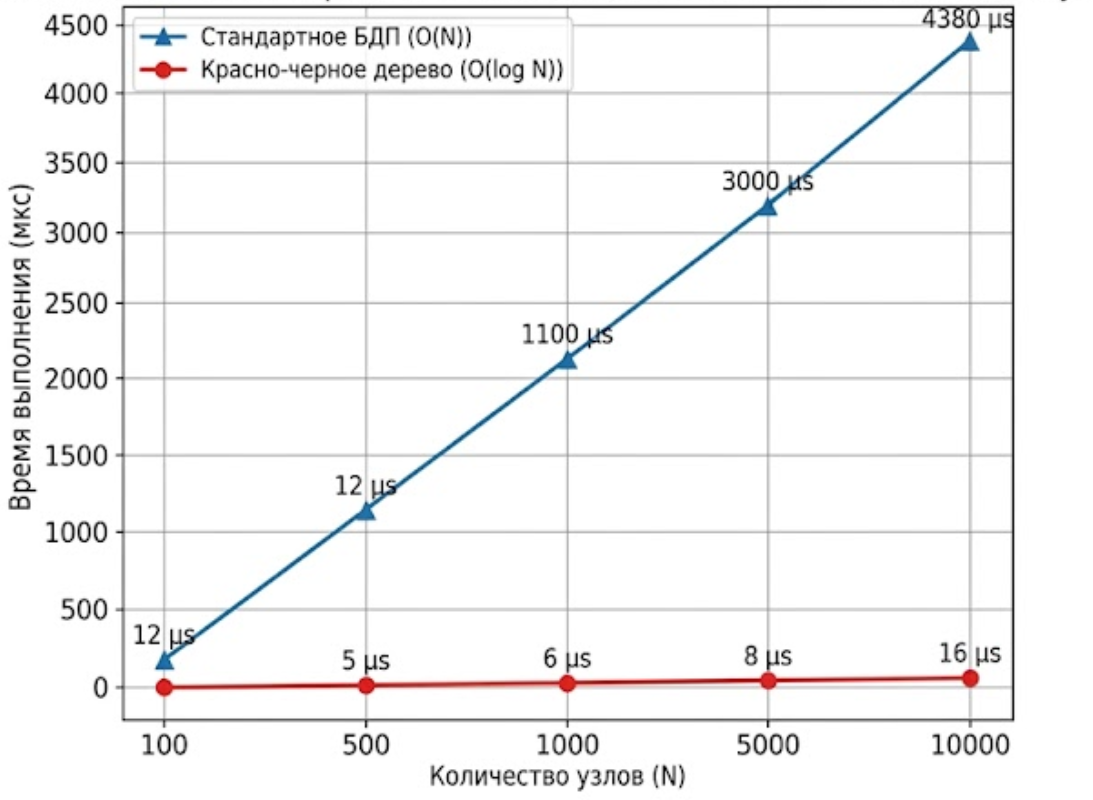
\includegraphics[width=0.65\textwidth]{img1}
\end{center}
\end{figure}

Для понимания внутренней структуры распределения памяти на рисунке~\ref{fig:tree_structure} показана схема размещения узлов в адресном пространстве процесса Linux после проведения балансировки.

\begin{figure}[h!]
\caption{Логическая структура красно-черного дерева и схема перестройки указателей в памяти процесса при левом повороте}
\label{fig:tree_structure}
\begin{center}
    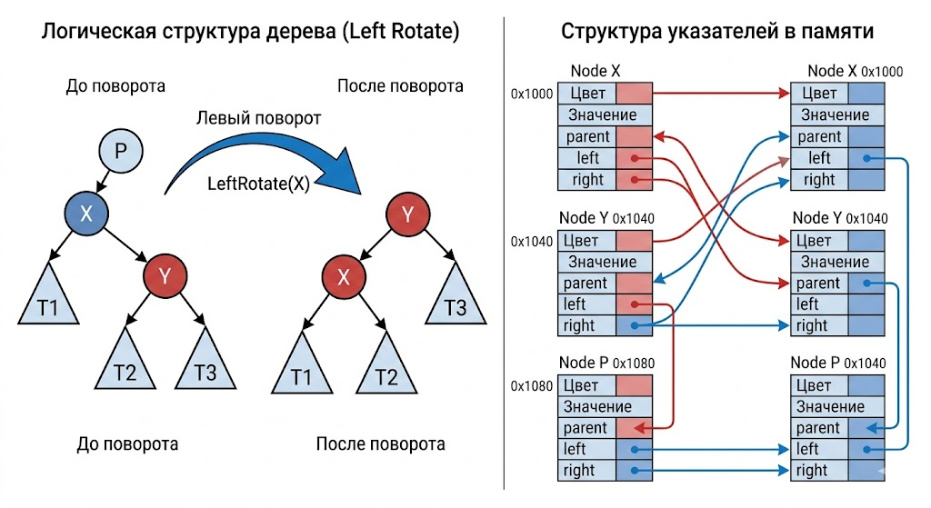
\includegraphics[width=0.75\textwidth]{img2}
\end{center}
\end{figure}

\conclusion

В ходе выполнения отчетной работы были успешно изучены механизмы функционирования самобалансирующихся систем поиска данных. Разработанная программная реализация на языке C++ продемонстрировала высокую стабильность и корректность выполнения структурных преобразований при модификации дерева. Проведенное автоматизированное тестирование полностью подтвердило соответствие полученных практических результатов теоретическим оценкам временной сложности алгоритма.

% Отобразить все источники. Даже те, на которые нет ссылок.
% \nocite{*}

\bibliographystyle{ugost2003}
\bibliography{thesis}

% Окончание основного документа и начало приложений Каждая последующая секция
% документа будет являться приложением
\appendix

\end{document}
